\item \points{20} {\bf Binary Classification: Experimenting with Activation Functions}\\~\\
\textbf{Note: }Although this problem is related to neural networks, we have specifically chosen this problem to allow you to practice the mathematical prerequisites for XCS229i, the loss-minimization framework, and the gradient descent update rules. You are not expected to know the architecture of neural networks until problem set 4 where it will be covered in more detail.\\~\\

Let $X = \{x^{(1)}, \cdots, x^{(\nexp)}\}$ be a dataset of $\nexp$ samples with 2 features, i.e $\xsi \in \R^2$. The samples are classified into 2 categories with labels $\ysi \in \{0, 1\}$. A scatter plot of the dataset is shown in Figure $\ref{fig:nn_plot}$:
\begin{figure}[htbp]
    \centering
    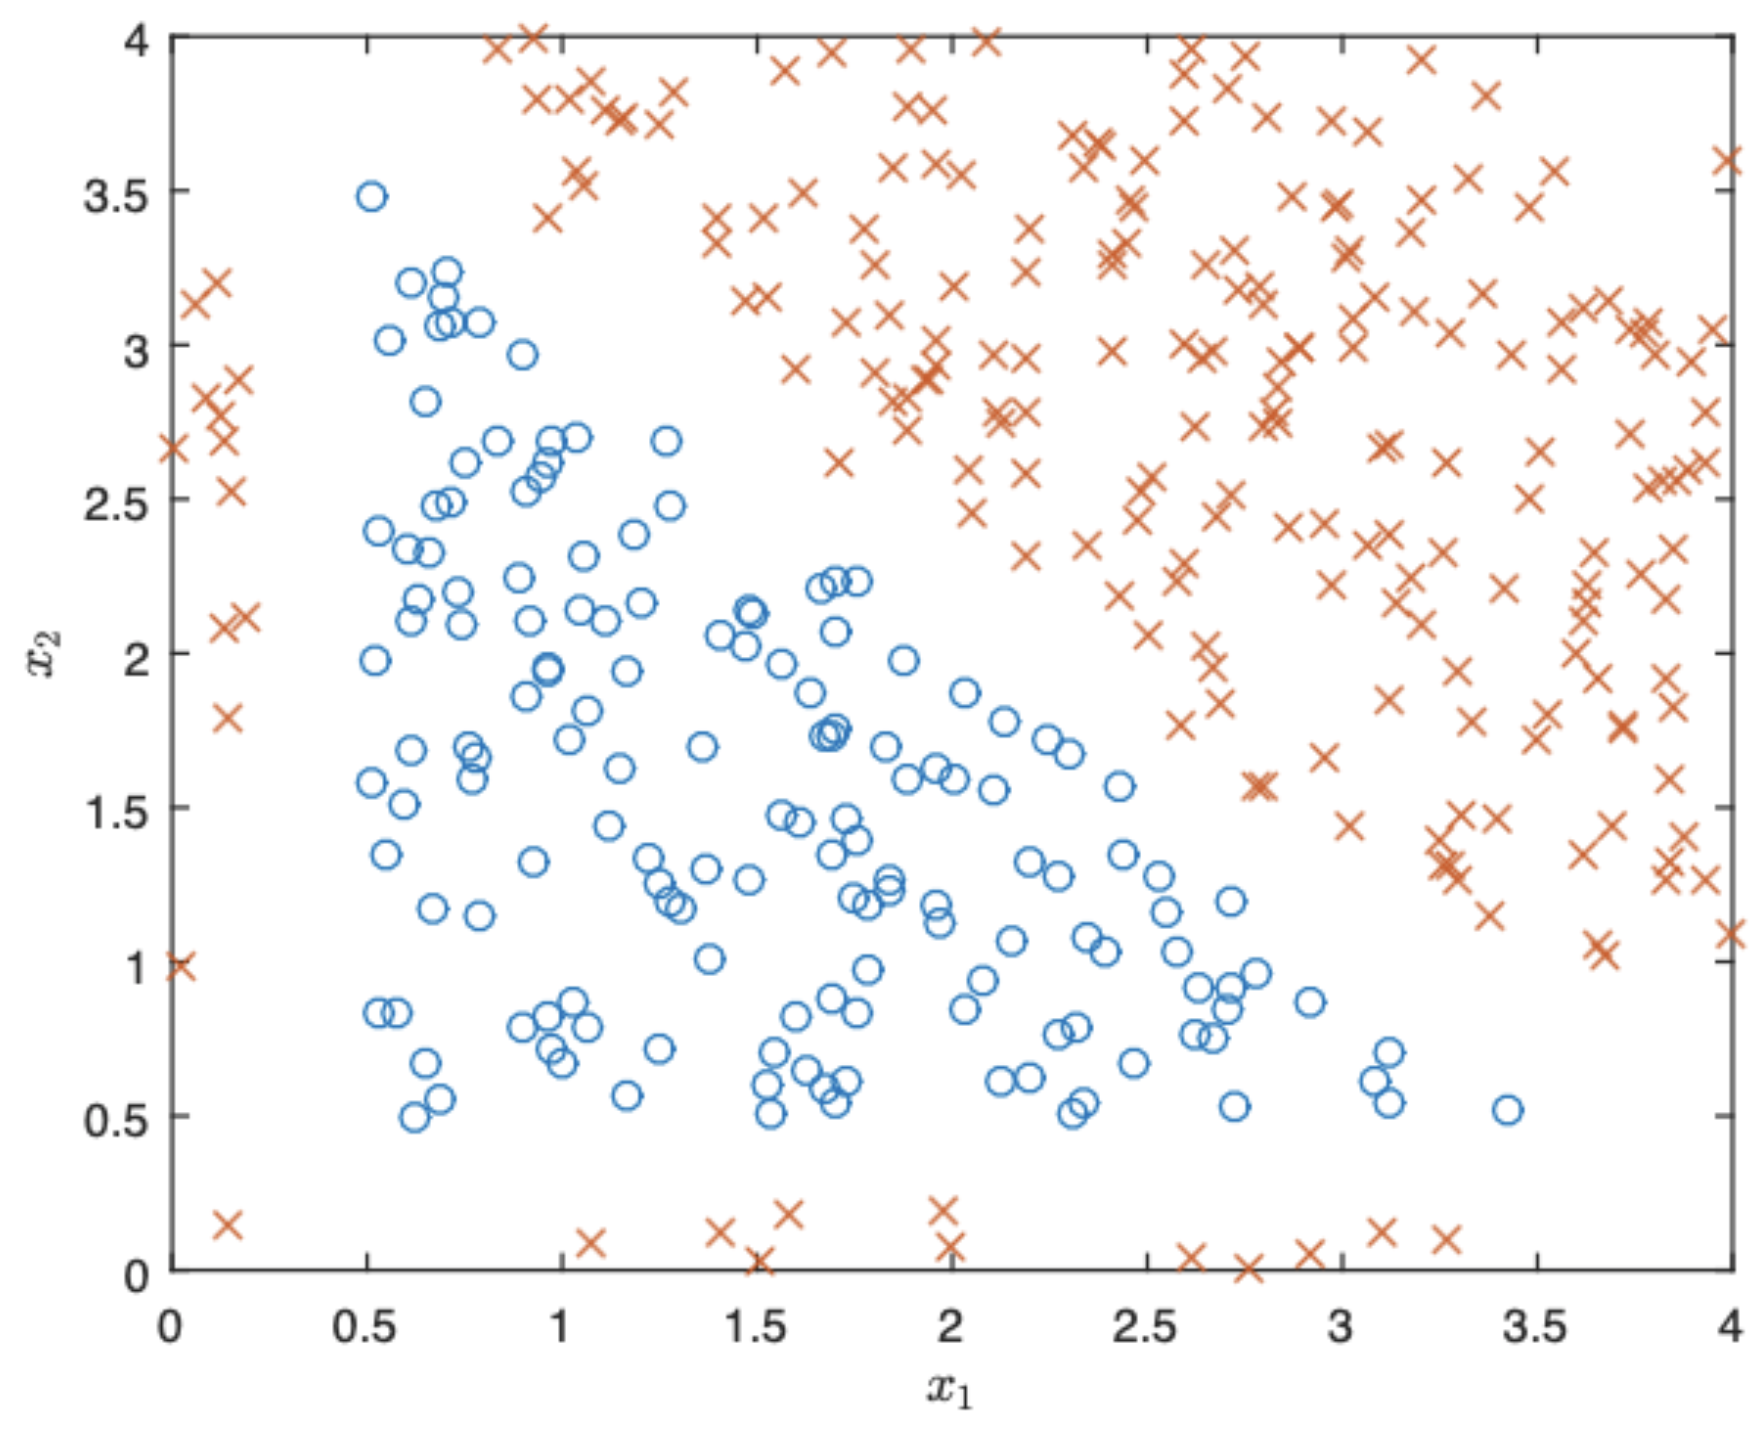
\includegraphics[scale=0.3]{simple_nn/nn_plot.png}
    \caption{Plot of dataset $X$.}
    \label{fig:nn_plot}
\end{figure}

The examples in class $1$ are marked as as ``$\times$" and examples in class $0$ are marked as ``$\circ$". We want to perform binary classification using a simple neural network with the architecture shown in Figure $\ref{fig:nn_arc}$:
\begin{figure}[htbp]
    \centering
    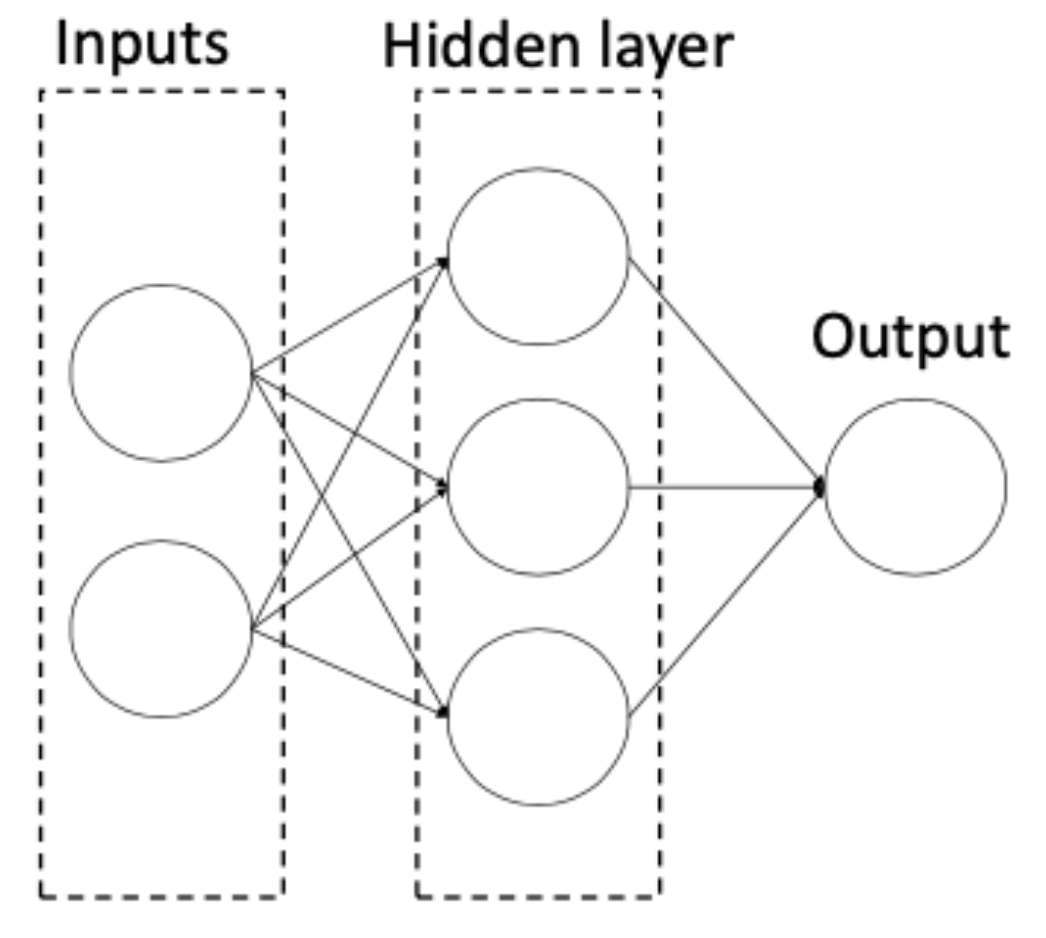
\includegraphics[scale=0.3, clip]{simple_nn/nn_architecture.png}
    \caption{Architecture for our simple neural network.}
     \label{fig:nn_arc}
\end{figure}

Denote the two features $x_1$ and $x_2$, the three neurons in the hidden layer $h_1, h_2$, and $h_3$, and the output neuron as $o$. Let the weight from $x_i$ to $h_j$ be $w_{i, j}^{[1]}$ for $i \in \{1, 2\}, j \in \{1, 2, 3\}$, and the weight from $h_j$ to $o$ be $w_{j}^{[2]}$. Finally, denote the intercept weight for $h_j$ as $w_{0, j}^{[1]}$, and the intercept weight for $o$ as $w_{0}^{[2]}$. For the loss function, we'll use average squared loss instead of the usual negative log-likelihood:
$$l = \frac{1}{\nexp}\sum_{i=1}^{\nexp} \left(o^{(i)} - \ysi\right)^2,$$
where $o^{(i)}$ is the result of the output neuron for example $i$.

\begin{enumerate}
  \item \subquestionpoints{5}
Suppose we use the sigmoid function as the activation function for $h_1, h_2, h_3$ and $o$.
What is the gradient descent update to $w_{1, 2}^{[1]}$, assuming we use a learning rate of $\alpha$?
Your answer should be written in terms of $\xsi$, $o^{(i)}$, $\ysi$, and the weights.\\

{\bf BEGIN PROOF HERE}\\

Let $g$ denote the sigmoid function $g(x) = \frac{1}{1 + e^{-x}}$, and $h^{(i)}_j$ denote the output of hidden neuron $h_j$ for sample $i$. For shorthand, we denote $\vec{w_j}^T\xsi = w_{1, j}^{[1]}x_1^{(i)} + w_{2, j}^{[1]}x_2^{(i)} + w_{0, j}^{[1]}$ for $j \in \{1, 2, 3\}$, and $\vec{w_o}^Th^{(i)} = w_{1}^{[2]}h^{(i)}_1 + w_{2}^{[2]}h^{(i)}_2 + w_{3}^{[2]}h^{(i)}_3 + w_{0}^{[2]}$. Using chain rule, we have
\begin{flalign*}
    \frac{\partial l}{\partial w_{1, 2}^{[1]}} &= & & & & & & & &\\[50pt]
    \frac{\partial (o^{(i)})}{\partial w_{1, 2}^{[1]}} &= & & & & & & & &\\[50pt]
    \frac{\partial (h^{(i)}_2)}{\partial w_{1, 2}^{[1]}} &= & & & & & & & &\\[50pt]
\end{flalign*}
Combining everything, we have
\begin{flalign*}
    \frac{\partial l}{\partial w_{1, 2}^{[1]}} = & & & & & & & &\\[50pt]
\end{flalign*}
and the update rule is \\[50pt]
{\bf END PROOF}\\

\ifnum\solutions=1 {
  \input{simple_nn/01-sigmoid_sol}
} \fi

  \item \subquestionpoints{8} Now, suppose instead of using the sigmoid function for the activation function for $h_1, h_2, h_3$ and $o$, we instead used the step function $f(x)$, defined as
\begin{align*}
f(x) = \begin{cases}
    1, x > 0 \\
    0, x \le 0
    \end{cases}
\end{align*}

Is it possible to have a set of weights that allow the neural network to classify this dataset with 100\% accuracy?

If it is possible, please provide a set of weights that enable 100\% accuracy as a table shown below

If it is not possible, please explain your reasoning in the writeup.

\textbf{Hint 1:} There are three sides to a triangle, and there are three neurons in the hidden layer.

\textbf{Hint 2:} A solution can be found where all weight and bias parameters take values only in $\{-1, -0.5, 0, 1, 3, 4 \}$. You are free to come up with other solutions as well.

\begin{table}[h]
\centering
\begin{tabular}{ |c||c|c||c|c||c|c||c|c|}
\hline
Neuron & Bias & Value &  Weight & Value & Weight & Value & Weight & Value\\
\hline
$h_1$ & $w_{0,1}^{[1]}$ &  & $w_{1,1}^{[1]}$ &  & $w_{2,1}^{[1]}$ &   & - & -\\
\hline
$h_2$ & $w_{0,2}^{[1]}$ &  & $w_{1,2}^{[1]}$ &  & $w_{2,2}^{[1]}$ &   & - & -\\
\hline
$h_3$ & $w_{0,3}^{[1]}$ &  & $w_{1,3}^{[1]}$ &  & $w_{2,3}^{[1]}$ &   & - & - \\
\hline
$o$ & $w_{0}^{[2]}$ &  & $w_{1}^{[2]}$ &  & $w_{2}^{[2]}$ &  & $w_{3}^{[2]}$ &  \\
\hline
\end{tabular}
\end{table}

\ifnum\solutions=1 {
  \input{simple_nn/02-step_function_sol}
} \fi

  \item \subquestionpoints{7} Let the activation functions for $h_1, h_2, h_3$ be the linear function $f(x) = x$ and the activation function for $o$ be the same step function as before.


Is it possible to have a set of weights that allow the neural network to classify this dataset with 100\% accuracy?

If it is possible, please provide a set of weights that enable 100\% accuracy as a table shown below

If it is not possible, please explain your reasoning in the writeup.

\textbf{Hint:} The hints from the previous sub-question might or might not apply.

\begin{table}[h]
\centering
\begin{tabular}{ |c||c|c||c|c||c|c||c|c|}
\hline
Neuron & Bias & Value &  Weight & Value & Weight & Value & Weight & Value\\
\hline
$h_1$ & $w_{0,1}^{[1]}$ &  & $w_{1,1}^{[1]}$ &  & $w_{2,1}^{[1]}$ &   & - & -\\
\hline
$h_2$ & $w_{0,2}^{[1]}$ &  & $w_{1,2}^{[1]}$ &  & $w_{2,2}^{[1]}$ &   & - & -\\
\hline
$h_3$ & $w_{0,3}^{[1]}$ &  & $w_{1,3}^{[1]}$ &  & $w_{2,3}^{[1]}$ &   & - & - \\
\hline
$o$ & $w_{0}^{[2]}$ &  & $w_{1}^{[2]}$ &  & $w_{2}^{[2]}$ &  & $w_{3}^{[2]}$ &  \\
\hline
\end{tabular}
\end{table}
\ifnum\solutions=1 {
  \input{simple_nn/03-linear_sol}
} \fi


\end{enumerate}
